% SyncBox manual - Maintenance
% Written by Christopher Thomas.
%
% Copyright (c) 2021 by Vanderbilt University. This work is released under
% the Creative Commons Attribution-ShareAlike 4.0 International License.

\chapter{Maintenance}
\label{sect-maint}

From time to time, new versions of the {\projectname} firmware are released.
These can be flashed using the ``\texttt{avrdude}'' utility, which is
bundled with the Arduino development environment or may be downloaded
on its own.

To use ``\texttt{avrdude}'', plug in the {\projectname}, determine what the
name of the Arduino's USB serial device is, bring up a ``command terminal''
window, navigate to the directory with the firmware file, and type:

\texttt{avrdude -c stk500 -p m2560 -P {\bfseries (device)}
-D -U flash:w:{\bfseries (firmware file)}}

For a firmware file named ``\texttt{usesyncbox-latest.hex}'', and a
USB serial device called ``\texttt{/dev/ttyACM0}'', the result will be similar
to the following:

\begin{center}
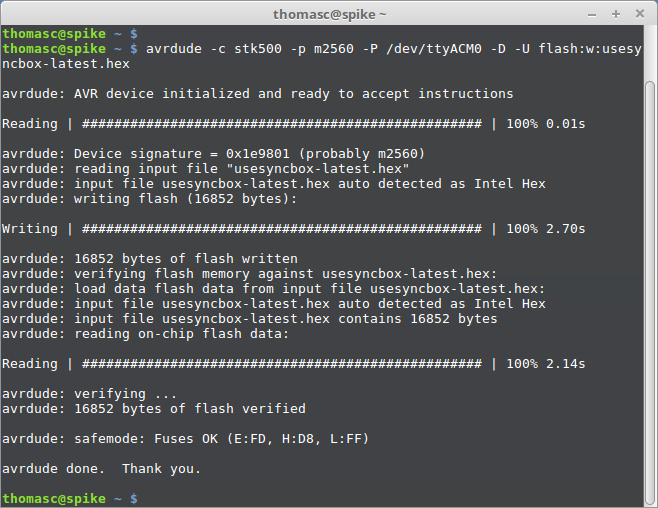
\includegraphics[height=3in]{screenshots/avrdude-linux.png}
\end{center}

The names of USB serial devices vary widely from operating system to 
operating system and version to version. Consult appropriate documentation 
to determine how to find the {\projectname}'s USB serial device on your
operating system.

\section{Using \texttt{avrdude} On Linux, Windows, and MacOS}

While \texttt{avrdude} can be installed as a stand-alone package, an easy and
reliable way to install it is to install the ``Arduino'' IDE (found at:
\verb|https://www.arduino.cc|). This will install several things:
\begin{itemize}
\item The Arduino development environment.
\item The \texttt{avr-gcc} compiler and its libraries.
\item The \texttt{avr-binutils} toolchain used with \texttt{avr-gcc}.
\item The \texttt{avrdude} program for flashing AVR-based boards.
\end{itemize}

Various quirks show up on each operating system:
\begin{itemize}

\item Under Linux, you may have to add a ``udev rules'' file in /etc/udev/ to
get Arduino boards detecting and connecting properly. The Arduino IDE package
\textit{should} set this up for you.

\item Under Windows 10, neither \texttt{avrdude} nor its configuration file
will be on path by default. To use it, first find out where it was installed,
and then either type the full path name ahead of the command or add the
relevant directory to the path.
\begin{itemize}
\item To find out where \texttt{avrdude} was installed, look for an
``Arduino'' shortcut on the desktop. Right-click it to edit its properties;
this will tell you what directory the Arduino binary is in. Open the
top-level directory in that tree, and tell Windows to search that folder
to find ``avrdude''. This will bring up the directory with \texttt{avrdude}
in it, which should also contain the ``\texttt{avrdude.conf}'' configuraton
file.
\item To set the path in Windows 10, go to ``control panel'', ``system'',
``advanced system settings'', ``advanced'' tab, ``environment variables''.
Under ``user variables'', select ``path'' and click ``edit''. Add the
directory as a new entry in the list.
\end{itemize}
\item To run \texttt{avrdude} from the command line under Windows, type the
following (as one line):

\texttt{(avrdude path)/avrdude -C (avrdude path)/avrdude.conf
-c stk500 -p m2560 -P (serial port)
-D -U flash:w:(firmware file including its path)}

\item Under MacOS, \fixme{Information goes here.}

\end{itemize}

%
% This is the end of the file.
